% !Mode:: "TeX:UTF-8" 

\section{国内外在该方向的研究现状及分析}
\subsection{国内外研究现状}

语义依存分析是一个新兴课题,虽然已经引起了许多研究者的关注,但是相关的数据集和研究工作相比分词、词性标注等历史悠久的任务都比较有限,而国内的研究更是非常少,因此这里将国内外的研究现状总结到一起描述。

语义依存树与句法依存树主要的区别在于依存弧上的标签不同,这源自于两种任务目标上的区别。因此语义依存树的分析基本可以沿用句法依存分析方法,对于后者目前已经存在大量的研究工作,目前应用最多的主要可以分为两大类:基于转移(Transition-based)和基于图(Graph-based)的依存分析。基于图的算法将依存分析转换为在有向完全图中求解最大生成树的问题,是基于动态规划的一种图搜索算法。该算法由\citeayu{mcdonald-crammer-pereira:2005:ACL}提出,是一种全局最优的搜索算法。\citeayu{yamada2003statistical} 提出的基于转移的依存分析算法将句子的解码过程建模为一个转移序列的构造过程。其依存分析模型的目标是通过学习得到一个能够准确的预测下一步转移动作的分类器。

语义依存图与句法依存树除了上述的依存弧标签不同之外,结构上也有所差异。语义依存图打破了传统的依存树结构,允许多父节点的存在(在依存树中一个词只能有一个父节点),因此能够刻画句中词之间更丰富的语义关系。但多父节点的存在同时也使得对语义依存图的分析更具挑战性。目前对语义依存图的分析工作主要使用的方法都是对上述基于转移和基于图的依存分析方法的扩展。下面我们首先简要介绍目前国内外的语义依存图数据集,然后分别对基于转移和基于图的语义依存图分析工作进行总结。

\subsubsection{语义依存图数据集}

目前国内的语义依存图数据集只有由哈工大社会计算与信息检索研究中心(HIT-SCIR)和北京语言大学合作标注的 SemEval-2016 Task 9 中文语义依存图数据集\cite{che-EtAl:2016:SemEval}。为了解决 SemEval-2012 Task 5 语义依存树数据集\cite{che-EtAl:2012:STARSEM-SEMEVAL}中语义关系彼此易混淆、语义关系数量太大、刻画语义不全面等问题,在中文语义依存图数据集中用依存图结构代替依存树。形式上类似于依存句法结构,但必要时突破树形结构(BH-SDP-v2标注体系)。这样的突破使得对连动、兼语、概念转位等汉语中常见的现象的分析更全面深入,当然这也给依存分析器的构建带来了很大的难度,因为任何词都可能有多个父节点。图~\ref{fig:sem16diff}直观地展示了语义依存树与依存图的区别。

\begin{figure}[tbhp]
	\centering
	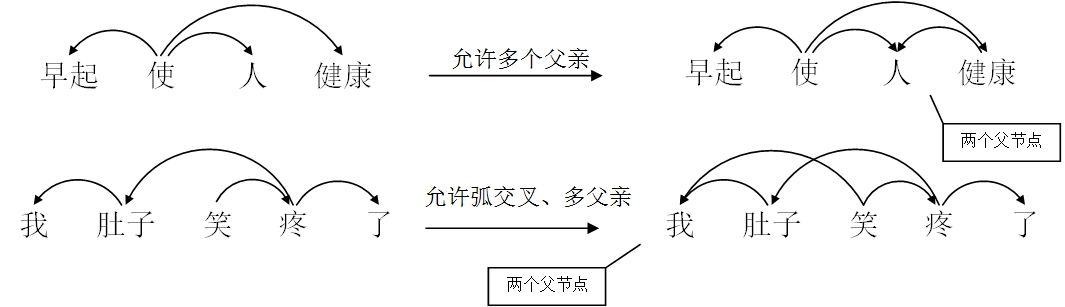
\includegraphics[width=85mm]{picture/sem16diff.jpg}
	\caption{中文语义依存树与语义依存图对比示例}
	\label{fig:sem16diff}
\end{figure}

BH-SDP-v2标注体系压缩了语义关系类型的数量,重新组织并缩减了语义关系,将关系分为主要语义角色、事件关系、关系标记,从而减少不必要的类间关系混淆。语义关系在保留了一般语义关系、反关系基础上,还增加了嵌套关系,用来标记一个事件降级充当了另一个事件的成分。SemEval-2016 Task 9 中文语义依存图数据集中包含10068句新闻语料和15000句课文句子。新闻句子平均长度是31个词,课本句子平均长度是14个词。该数据集被用于 SemEval-2016 Task 9 国际公开评测上。

\begin{figure}[tb]
	\centering
	\small
	\subfigure[DM]{\label{fig:sem15-dm}
		\begin{dependency}[theme = simple,label style={font=\bfseries,thick}]
			\begin{deptext}[column sep=0.3em]
				Last \& week \& , \& shareholders \& took \& their \& money \& and \& ran \\
			\end{deptext}
			\deproot[edge unit distance=2.8ex]{5}{top}
			\depedge{1}{2}{arg1}
			\depedge{2}{5}{loc}
			\depedge{5}{4}{arg1}
			\depedge{5}{7}{arg2}
			\depedge{5}{9}{\_and\_c}
			\depedge{6}{7}{poss}
			\depedge[edge start x offset = 6pt]{9}{4}{arg1}
			%\depedge[edge start x offset=-4pt, edge end x offset=-3pt]{8}{9}{conj}
		\end{dependency}
	}
	
	\subfigure[PAS]{\label{fig:sem15-pas}
		\begin{dependency}[theme = simple,label style={font=\bfseries,thick}]
			\begin{deptext}[column sep=0.3em]
				Last \& week \& , \& shareholders \& took \& their \& money \& and \& ran \\
			\end{deptext}
			\deproot[edge unit distance=2.8ex]{8}{top}
			\depedge{1}{2}{arg1}
			\depedge{2}{8}{arg1}
			\depedge{5}{4}{arg1}
			\depedge{5}{7}{arg2}
			\depedge{6}{7}{arg1}
			\depedge{8}{5}{coord}
			\depedge{8}{9}{coord}
			\depedge[edge start x offset = 6pt]{9}{4}{arg1}
		\end{dependency}
	}
	
	\subfigure[PSD]{\label{fig:sem15-psd}
		\begin{dependency}[theme = simple,label style={font=\bfseries,thick}]
			\begin{deptext}[column sep=0.3em]
				Last \& week \& , \& shareholders \& took \& their \& money \& and \& ran \\
			\end{deptext}
			\deproot[edge unit distance=2.8ex]{5}{top}
			\deproot[edge unit distance=2.8ex]{9}{top}
			\depedge{2}{1}{rstr}
			\depedge{5}{2}{twhen}
			\depedge{5}{4}{act}
			\depedge{5}{7}{pat}
			\depedge{7}{6}{app}
			\depedge{8}{5}{conj}
			\depedge[edge start x offset=-4pt, edge end x offset=-3pt]{8}{9}{conj}
			\depedge[edge start x offset=3pt]{9}{4}{act}
			\depedge[edge start x offset=3pt]{9}{2}{twhen}
		\end{dependency}
	}
	\caption{广义语义依存图三种标注体系示例}
	\label{fig:sem15}
	
\end{figure}

国外的语义依存图数据集主要是SemEval-2015 Task 18广义(Broad-Coverage)语义依存图数据集。
其目标是获取句子内部所有实词之间的谓词论元关系,即获取表示该句子含义的语义结构。构建该数据库的目的是寻找更具普适性的图结构,从而提供对“Who did what to whom”等问题更直接的分析方式。
该语料库中使用了三种不同的标注体系(图~\ref{fig:sem15}给出了三种标注的例子),分别是:

\begin{enumerate}
	\item \textbf{DM (DELPH-IN MRS-Derived Bi-Lexical Dependencies)}
	该语义依存图标注来源于参考LinGO英文资源语法(English Resource Grammar)给出的句法、语义信息进行人工重标注的DeepBank语料。
	
	\item \textbf{PAS (Enju Predicate–Argument Structures)}
	Enju树库和分析器来源于对宾州树库的HPSG形式自动标注。PAS语义依存图是直接从Enju树库中抽取的,没有进行内容转换。
	
	\item \textbf{PSD (Prague Semantic Dependencies)}
	布拉格捷克语-英语依存树库(Prague Czech-English Dependency Treebank)是包括宾州树库华尔街日报部分及其捷克语翻译的依存树的语料库。PSD语义依存图是从该树库的构造语法标注层(tectogrammatical annotation layer)中抽取出来的。
\end{enumerate} 

该数据集中包括英语、中文和捷克语的语料。其中英语部分来自宾州树库(PTB)华尔街日报和布朗部分,包括35657句训练语料、1410句同领域测试语料及1849句不同领域(来自布朗部分)测试语料,拥有DM、PAS和PSD三种标注规范的语义依存图。中文部分来自中文宾州树库(CTB 7.0),包括31113句训练语料和1670句同领域测试语料,只有PAS规范的标注。捷克语部分来自宾州树库华尔街日报部分的捷克语翻译,包括42076句训练语料、1670句同领域测试语料及5226句不同领域测试语料,只有PSD规范的标注。 
该语料的英语部分首先用于 SemEval-2014 Task 8 评测\cite{oepen-EtAl:2014:SemEval}。此后的 SemEval-2015 Task 18 评测任务\cite{oepen-EtAl:2015:SemEval}中,该语料库又加入了中文和捷克语部分语料。

除此之外,还有一些数据集与语义依存图在结构或内容上有相似之处,包括 CoNLL-2009 数据集\cite{hajivc-EtAl:2009:CoNLL-2009-ST}的语义角色标注(Semantic Role Labeling)部分、CCD(CCG Dependencies)\cite{hockenmaier2007ccgbank}、AMR(Abstract Meaning Representation)数据集\cite{W13-2322}、丹麦语依存树库\cite{kromann2003danish}(DDT)和HPSG树库\cite{miyao2005corpus}等。
其中前两个属于语义角色标注范畴,其目的是找出句中一些谓词与其论元之间的关系,因此该任务一般分为两步,第一步是识别出句中的谓词,第二步才是找到每个谓词对应的论元。这里所说的谓词,一般来说指的是动词和名词。而语义依存分析的目的是找到句中所有词之间的语义关系,对词的种类没有限制,因此不需要进行上述的第一步。从两个任务目的上的不同能够发现,语义依存分析能提供一个句子更全面的语义信息。
AMR属于语义网络(Semantic Network),其中图节点表示的是语义概念,不需要与句中的词一一对应。而语义依存图则用有向弧直接表示的句中词之间的语义关系。此外,AMR目前只有英文数据,在中文上没有与之类似的数据集。
丹麦语依存树库和HPSG树库本质上来说也属于依存句法树库,但由于其中也包含一些图结构的依存句法表示,因此在语义依存图没有提出之前,一些对图结构分析算法的研究是在这些数据集上进行的,这些方法对我们也有一定的启示作用。

\subsubsection{基于转移的分析方法}

在基于转移的依存图分析方向上,\citeayu{sagae2008shift}发表了通过向转移系统中增加新的转移动作实现基于转移的依存图分析的先驱性工作。在传统的基于转移的依存树分析系统中,由于每个词只有一个父节点,因此一旦找到一个词的父节点就要将该词从系统中删除(LEFT-REDUCE和RIGHT-REDUCE动作),Sagae等人在转移系统中加入两个新的生成依存弧的动作(LEFT-ATTACH和RIGHT-ATTACH),只生成依存弧而不删除词,从而实现了多父节点结构的生成。他们在丹麦语依存树库和HPSG树库两个含有图结构的依存句法树库中进行了实验。此后该方向上的研究工作主要都集中在通过修改转移系统处理依存图结构。增加两个新的动作是一个最直观的解决依存图分析问题的方法,但是新增的两个动作只生成依存弧,不改变转移系统状态,在执行这两个动作前后转移系统的状态是基本不变的,这也就导致了从当前状态中提取出的用于预测下个转移动作的特征也是基本相同的,这会影响分类器预测的准确性,从而降低系统的整体性能。
\citeayu{Titov:2009:OGP:1661445.1661696}提出了另一种转移系统,在生成弧的同时不改变系统中的词,而是用独立的REDUCE动作删除已经无用的词,同时利用SWAP动作改变系统中词的顺序。

\citeayu{Zhang:2016:TPD:3030588.3030589} 提出了两种新的转移系统,第一种在线重排序(Online re-ordering)系统与Titov的系统类似,第二种基于双栈的(Two-Stack-Based)系统拥有一个额外的栈,用于保存从正在处理词的栈中暂时移除的词,通过MEM和RECALL两个动作实现向该额外的栈中保存词和从该栈中取词。除了转移系统外,基于转移的依存分析中十分重要的另一个部分就是用于在给定转移状态下预测下一个转移动作的分类器。Zhang等人在实验中也发现如果转移动作集合中存在只生成依存弧而不改变转移系统的动作,会影响分类器准确性。为了解决这一问题,他们将与生成依存弧有关的动作(NO、LEFT和RIGHT,分别表示不生成弧,生成向左或向右的弧)和改变转移状态的动作(SHIFT、REDUCE、SWAP等)两两组合,在最终的系统中使用组合后动作,保证了每个动作都会改变转移系统状态,成功提高了系统性能。

\subsubsection{基于图的分析方法}

在基于图的依存分析方向上,\citeayu{mcdonald2006online}首先提出了利用近似Eisner算法\cite{eisner1996three}解决基于图的依存分析中多父节点的生成的方法。他们首先使用原始Eisner算法生成一个投射树(依存弧存在交叉的树),然后对树中的边逐条替换,替换时允许出现多父节点,保留使整体评分增加的替换,从而生成图结构。McDonald等人也在丹麦语依存树库上进行了实验。这种方法本质上来说只是在传统的依存树分析算法得到的结果的基础上进行后处理,将树结构改成图结构,面对较复杂的图结构依然不能算是一个很好的解决方案。

\citeayu{martins2014priberam}提出了一种利用二阶特征的方法,在单个弧的一阶特征基础上,增加了连续兄弟节点、连续多父节点等二阶特征,使用$AD^3$算法\cite{martins2014ad3}进行解码,实现了依存图的预测。$AD^3$算法是一种基于对偶分解的近似离散优化算法。由于这里采用的分解方式不是以弧为因子的(arc-factored),各结构之间存在重叠,所以需要使用该算法进行解码。与McDonald等人的方法相比,该方法能够直接预测出图结构,而不是通过对依存树的后处理生成依存图。

\citeayu{peng-thomson-smith:2017:Long}利用了广义语义依存图语料库中英语部分有三种不同标注的特点,采用了多任务学习方法,仅用一阶特征就在该数据集上取得了当时最好结果。不仅如此,他们还借鉴了基于图的依存树分析研究中对神经网络的成功应用\cite{TACL885},将句中每个词的词向量输入双向长短时记忆网络(Bidirectional Long-Short Term Memory, Bi-LSTM),用其隐层输出作为每个词的表示,然后利用多层感知器(Multi-Layer Perceptron, MLP)计算每条候选弧的分数。通过这种方法,他们的模型即使不使用多任务学习方法,也有很好的表现。


\subsection{国内外文献综述的简析}
\subsubsection{现有工作的总结及其不足}
\label{drawback}

由于语义依存图的概念才提出不久,中文及其他语言上的语义依存图相关数据集构建工作也是近几年才初步完成,语料有限,目前为止国内外对于语义依存图分析的研究工作还比较少。因此,我们不但调研了专门研究语义依存图分析的工作,也从此前对于句法依存图等图结构分析的研究工作中获取灵感。总的来说,目前基于转移的依存分析方法和基于图的依存分析方法都开辟出了各自对图结构进行分析的道路。

在基于转移的分析方法中,目标依存结构是通过在包括待分析句子信息的转移系统(Transition System)中执行一系列的类似移进、规约的转移动作修改转移状态(转移系统中各部分的状态)来生成的,其最终目的是训练一个给定当前转移状态能够预测出接下来要执行的转移动作的分类器。因此,在这类方法中生成依存图的最大困难来自于每个词的父节点由原来的一个变成了任意多个,导致分类器难以判断何时对一个词进行规约。针对这一问题一般的解决办法是修改转移系统,提出新的转移动作替代或补充原有转移动作,从而增强转移系统的处理能力,使其可以产生依存图结构。因此如何设计或修改转移系统,就成为了基于转移的分析方法中一个十分重要的研究问题。此外,由于这类方法的核心是用于预测转移动作的分类器的训练,而分类器预测的依据则是当前的转移状态,因此如何更好、更快、更全面地获得当前转移状态的信息将其作为分类器的分类依据就成为了这类方法中另一个十分值得研究的问题。

在基于图的分析方法中,首先要将目标分成许多子结构,计算出所有可能的子结构的分数。分解方式有很多种,以一条弧为单位的分解称为一阶分解(first-order factorization),以两条弧一组为单位进行的分解称为二阶分解(second-order factorization)。然后利用动态规划算法计算出总分最大的子结构组合。
当分析目标是依存树时,一般使用最大生成树(Max Spanning Tree)算法。在面对依存图结构时,由于每个词的父节点个数由一个变为任意多个,而依存图又有非投射性(弧之间存在交叉),原来的动态规划算法不再适用,只能对每个子结构进行独立判断。如果使用了多种分解方式,则需要采用$AD^3$算法解决各子结构存在重叠时的解码问题。

上述两类方法中的绝大部分工作都使用了诸如线性模型、最大熵模型、结构化感知器等传统统计学机器学习方法。它们都是通过人工特征工程实现从环境中获取信息的,这样人工设计特征模板不但繁琐,需要该领域的专家知识,而且往往无法涵盖所有的信息,同时,对特征字符串的组合也会耗费大量时间。

近年来,模型融合(Model Ensemble)技术在依存句法分析领域已被证明十分有效,但是目前的模型融合方法不是利用多个不同模型的最终结果进行投票决定最终预测结构,就是对同一模型使用不同的随机初始化种子多次训练然后同时使用这些独立训练的模型进行预测。而且后者仅仅被应用在基于转移的依存分析中,并没有工作将这种模型融合方式应用于基于图的依存分析中。这两种模型融合方式虽然简单有效,但没有利用依存分析任务的特性,仅仅是把其它领域的模型融合方式简单搬运到依存分析领域,缺乏针对性。

作为一个新兴研究课题,中外文的语义依存图语料数量都十分有限,这给语义依存图分析研究的进行和高精度语义依存图分析器的训练都带来了巨大挑战。在这种情况下,更应该充分利用现有多种语言的语料资源,同时利用依存句法分析、语义角色标注等已有大量人工标注数据的相关任务帮助提高语义依存图分析器的精度。\citeayu{peng-thomson-smith:2017:Long}已经在SemEval-2015 Task 18英文广义语义依存图数据集上证明了通过多任务学习方法同时学习该数据集的三种标注体系能够有效提高最终的实验结果。但目前这方面的其它工作十分有限,仍有很大的研究空间。

\subsubsection{有待深入研究的问题}

与分词、句法分析等历史悠久的任务相比,语义依存图分析是一个十分年轻的任务,许多相关研究才刚刚起步,无论是在分析方法本身的研究上,还是在提高分析系统性能、利用多语言及其他任务数据的研究上,都有许多工作可以做。对于分析方法来说,基于转移的和基于图的两类依存图分析方法的研究都刚刚开始,孰优孰劣未有定论,因此这两类方法的研究都很有价值和意义。而在有了依存图分析方法之后,提出适应语义依存图任务特性的方法来提高系统性能则成为最重要的问题。另一方面,由于目前语义依存图语料较少,如何充分利用现有多种语言的语料资源以及依存句法分析、语义角色标注等相关任务的数据也是一个十分有意义的研究方向。因此,未来对于语义依存图分析的研究将集中在一下几个方面:

\begin{enumerate}
	\item \textbf{基于转移的分析方法}:在传统基于转移的依存树分析方法基础上,如何提出新的转移系统,解决分类器不知道何时对一个词进行规约的问题,使其能生成依存图结构,是基于转移的依存图分析方法的根本。在此基础上,研究如何使用新的信息抽取方式代替原来低效、繁琐的人工特征工程,从而更好、更快、更全面地获得当前转移状态的信息是十分有意义的
	
	\item \textbf{基于图的分析方法}:在基于图的分析方法中,第一步计算每个子结构的分数是至关重要的,因为此后使用解码算法得到的依存图结构完全是依赖于第一步中得出的分数的。所以在基于图的分析方法中如何从句子中获取更全面的信息帮助计算子结构的分数是很值得研究的。
	
	\item \textbf{利用模型融合技术提高系统性能}:模型融合已经在许多领域证明是一个简单有效的提高系统性能的方法。现有的在依存分析系统中利用模型融合技术的工作实现的仅仅是简单的最终结果投票融合或者是使用不同的随机初始化种子。这些方法并没有考虑到语义依存分析任务的特性,同时可解释性也不强。因此,如何设计一个符合语义依存分析任务特性,能够融合对不同维度信息进行建模的融合方法,将是十分重要的。
	
	\item \textbf{利用多语言、多领域数据}:随着深度学习技术在各领域取得的巨大成功,数据量往往与使用深度学习技术的系统性能成正比。由于语义依存图语料有限,如何充分利用现有多种语言的语料资源以及依存句法分析、语义角色标注等已有大量人工标注语料的相关任务数据也是一个十分有意义的研究方向。
	
\end{enumerate}




